\documentclass[xetex,mathserif,serif]{beamer}
\usepackage{polyglossia}
\setdefaultlanguage[babelshorthands=true]{russian}
\usepackage{minted}

\usetheme{SPbGU}

\setmainfont{FreeSans}
\newfontfamily{\russianfonttt}{FreeSans}

\definecolor{links}{HTML}{2A1B81}
\hypersetup{colorlinks,linkcolor=,urlcolor=links}

\title{Методика проведения учебных практик}
\subtitle{На кафедре системного программирования СПбГУ}
\author[Юрий Литвинов]{Юрий Литвинов \newline \textcolor{gray}{\small\texttt{yurii.litvinov@gmail.com}}}
\date{}

\begin{document}
{
\setbeamertemplate{footline}{}
% Лого университета или организации, отображается в шапке титульного листа
\begin{frame}
  
\includegraphics[width=1.4cm]{pictures/SPbGU_Logo.png}
\vspace{-35pt}
\hspace{-10pt}
\begin{center}
   \begin{tabular}{c}
        \scriptsize{Санкт-Петербургский государственный университет} \\
        \scriptsize{Кафедра системного программирования}
    \end{tabular}
\titlepage
\end{center}

\btVFill

\begin{center}
  \vspace{5pt}
  \scriptsize{Санкт-Петербург\\
                 2020}
  \end{center}

\end{frame}
}

    \section{Модель практики}

    \begin{frame}
        \frametitle{Что такое учебная практика}
        \begin{itemize}
            \item Знакомство студентов с реалиями профессиональной деятельности
            \item Цель --- применить полученные знания, ``прочувствовать'' их полезность, научиться целостному процессу работы
            \item Научно-исследовательская или программно-инженерная работа%
            \begin{itemize}
                \item Программирование с использованием программно-инженерных техник
                \item Оформление отчёта по практике
                \item Презентация результатов на защите перед комиссией
            \end{itemize}
            \item Тема индивидуальна, но допустимы и приветствуются командные работы
            \begin{itemize}
                \item Тема должна быть интересна кафедре (``программирование для программистов'')
            \end{itemize}
        \end{itemize}
    \end{frame}

    \begin{frame}
        \frametitle{Место практики в учебном плане}
        \begin{itemize}
            \item С начала второго курса
            \begin{itemize}
                \item За первый курс надо сделать из школьника младшего разработчика
                \item Навыки написания кода, ООП, модульное тестирование, системы контроля версий, непрерывная интеграция, основы архитектуры...
            \end{itemize}
            \item На втором курсе --- попробовать сделать что-то руками вне программы, параллельно с курсами по программированию
            \begin{itemize}
                \item Не требуется особая актуальность
            \end{itemize}
            \item На третьем курсе --- исследовательский или инженерный проект в составе команды, параллельно со спецкурсами
            \item На четвёртом курсе --- преддипломная практика, работа над ВКР
            \begin{itemize}
                \item ВКР по сути та же практика, только объёмнее и серьёзнее
            \end{itemize}
            \item Много зачётных единиц
        \end{itemize}
    \end{frame}

    \begin{frame}
        \frametitle{Что мы требуем}
        \begin{itemize}
            \item Текст отчёта --- порядка 5-7 страниц в 3-м семестре, порядка 25 в 6-м, порядка 30-40 для ВКР
            \begin{itemize}
                \item В формате, близком к научным статьям или техническим отчётам
                \item Текст проходит выборочное рецензирование одинарным слепым способом
            \end{itemize}
            \item Презентация примерно на 7 минут
            \item Код в репозитории, оформленный согласно принятым в сообществе практикам
            \begin{itemize}
                \item Также проверяется при рецензировании работы
            \end{itemize}
            \item Отзывы научного руководителя и консультанта
        \end{itemize}
    \end{frame}

    \begin{frame}
        \frametitle{Роли}
        \begin{itemize}
            \item Научный руководитель --- отвечает за текст и презентацию, помогает с методологией
            \item Консультант --- ставит задачу, помогает технически
            \begin{itemize}
                \item Научный руководитель и консультант ``играют на стороне студента против комиссии''
                \item Постоянное общение, демократичная творческая атмосфера
            \end{itemize}
            \item Куратор практики --- организует процесс, решает проблемы
            \item Комиссия --- слушает защиту, критикует работу
            \begin{itemize}
                \item Включает в себя представителя IT-компании
                \item Задача комиссии --- жёстко критиковать
            \end{itemize}
        \end{itemize}
    \end{frame}

    \begin{frame}
        \frametitle{Процесс}
        \begin{itemize}
            \item Сентябрь-октябрь --- выбор тем
            \begin{itemize}
                \item В основном темы от индустриальных партнёров, есть и кафедральные
            \end{itemize}
            \item Декабрь --- зачёт за осенний семестр (текст, отзывы, защита)
            \begin{itemize}
                \item Требуется постановка задачи, обзор и мысли по реализации
                \item На втором курсе практика может быть полугодовой, тогда требуется всё
            \end{itemize}
            \item Апрель --- предзащиты (для ВКР ещё и предпредзащиты)
            \item Май --- зачёт за весенний семестр (текст, отзывы, защита)
            \item За неделю до защит --- выборочное рецензирование текстов
            \item Как минимум раз в две недели коммуникация с научным руководителем
        \end{itemize}
    \end{frame}

    \section{Требования к отчёту}

    \begin{frame}
        \frametitle{Требования к отчёту}
        \begin{itemize}
            \item Титульный лист
            \item Оглавление
            \item Введение в предметную область
            \item Постановка задачи
            \item Обзор литературы, используемых технологий и существующих решений
            \item Описание предлагаемого решения 
            \begin{itemize}
                \item Архитектура (если применимо)
                \item Особенности реализации
                \item Апробация и/или эксперименты
            \end{itemize}
            \item Заключение
            \item Список литературы
        \end{itemize}
    \end{frame}

    \begin{frame}
        \frametitle{Название работы}
        \begin{itemize}
            \item Кратко, но понятно
            \item Должен быть понятен вклад
            \begin{itemize}
                \item Реализация, анализ, эксперимент, доказательство
                \item Специфично
            \end{itemize}
            \item Аббревиатуры только с квалифицирующим словом
        \end{itemize}
    \end{frame}

    \begin{frame}
        \frametitle{Введение}
        \begin{columns}
            \begin{column}{0.6\textwidth}
                \begin{itemize}
                    \item Известная информация, ``Background''
                    \item Неизвестная информация, ``Gap''
                    \begin{itemize}
                        \item Актуальность темы
                        \item Практическая значимость
                        \item Кому конкретно это надо
                    \end{itemize}
                    \item Кратко про подход к решению задачи, почему он приведёт к успеху (``Гипотеза'' и ``Подход'')
                \end{itemize}
            \end{column}
            \begin{column}{0.4\textwidth}
                \begin{center}
                    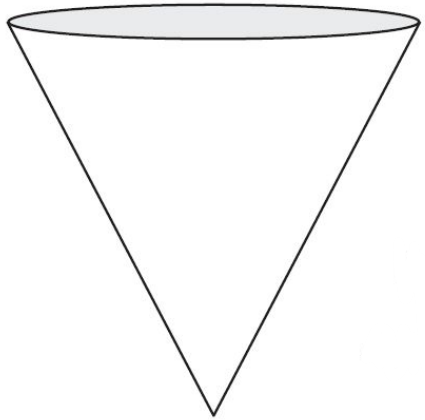
\includegraphics[width=\textwidth]{introductionCone.png}
                \end{center}
            \end{column}
        \end{columns}
    \end{frame}

    \begin{frame}
        \frametitle{Постановка задачи}
        \begin{itemize}
            \item Цель работы
            \begin{itemize}
                \item Одним предложением --- что конкретно надо сделать
            \end{itemize}
            \item Задачи
            \begin{itemize}
                \item Отчуждаемые
                \item Специфичные
                \item Решение которых приведёт к цели
                \begin{itemize}
                    \item Типовые задачи: выполнить обзор, спроектировать, реализовать, выполнить апробацию/эксперименты
                \end{itemize}
                \item Отдельно на осеннюю и весеннюю часть
            \end{itemize}
        \end{itemize}
    \end{frame}

    \begin{frame}
        \frametitle{Обзор}
        \begin{itemize}
            \item Обзор существующих решений
            \begin{itemize}
                \item Цель обзора, критерии отбора материалов, методика поиска
                \item Критерии сравнения
                \item Таблица с результатами
                \item Выводы
            \end{itemize}
            \item Обзор используемых чужих результатов
            \begin{itemize}
                \item  Всё, написанное и придуманное не в рамках работы --- в обзор
            \end{itemize}
            \item Должен соотноситься с темой работы
        \end{itemize}
    \end{frame}

    \begin{frame}
        \frametitle{Описание решения}
        \begin{itemize}
            \item Несколько разделов
            \begin{itemize}
                \item Желательно, чтобы разделы соответствовали списку задач
            \end{itemize}
            \item Аргументированное обоснование принятых решений и отказа от альтернатив
            \item Выбор инструментария (выбрали из чего и почему)
            \item Описание архитектуры, алгоритмов и т.п.
        \end{itemize}
    \end{frame}

    \begin{frame}
        \frametitle{Описание решения (2)}
        \begin{itemize}
            \item Рисунки и диаграммы, таблицы
            \begin{itemize}
                \item UML для описания архитектуры
                \item Подписи
                \begin{itemize}
                    \item Чужие рисунки --- со ссылкой на источник
                \end{itemize}
                \item Ссылки из текста
                \item Сквозная нумерация
            \end{itemize}
        \end{itemize}
    \end{frame}

    \begin{frame}
        \frametitle{Апробация/эксперименты}
        \begin{itemize}
            \item Цель раздела --- доказать, что получился содержательный результат
            \item Для технических работ --- описание опыта внедрения, опыта использования и отзывов пользователей
            \begin{itemize}
                \item Систематически, например, System Usability Score
            \end{itemize}
            \item Для ``научных'' работ --- эксперименты и сравнения с аналогами
            \begin{itemize}
                \item Статистическая обработка результатов
                \item Подписи к осям, единицы измерения
            \end{itemize}
            \item Для теоретических работ --- публикация
        \end{itemize}
    \end{frame}

    \begin{frame}
        \frametitle{Заключение}
        \begin{itemize}
            \item Перечисление результатов, выносимых на защиту
            \item Должно быть согласовано с постановкой задачи (вплоть до полного её повторения)
            \item Должно быть согласовано с текстом
            \begin{itemize}
                \item Никаких результатов из ниоткуда
            \end{itemize}
            \item Отчуждаемые и проверяемые результаты
            \item В осенних практиках также указываются планы на весну
        \end{itemize}
    \end{frame}

    \begin{frame}
        \frametitle{Литература}
        \begin{itemize}
            \item Cсылок примерно как страниц в работе
            \item Обязательно на каждый пункт ссылаться из текста
            \item Предпочтительно ссылаться на научные статьи или книги
            \item ГОСТ Р 7.0.5-2008
            \item Подстраничные сноски для ссылок на сайты, статьи на Хабре и т.д.
            \item Электронные источники в списке литературы допустимы (надо указывать дату обращения)
        \end{itemize}
    \end{frame}

    \begin{frame}
        \frametitle{Презентация, структура}
        \begin{itemize}
            \item Титульный слайд
            \item Введение (примерно 1 слайд)
            \item Постановка задачи (1 слайд)
            \item Обзор (примерно 1 слайд)
            \item Предлагаемое решение (примерно 1-2 слайда)
            \item Эксперименты/апробация (примерно 1 слайд)
            \item Результаты, выносимые на защиту (1 слайд) --- обязательно, последним слайдом
        \end{itemize}
    \end{frame}

    \begin{frame}
        \frametitle{Особенности}
        \begin{itemize}
            \item Никакого заимствования 
            \begin{itemize}
                \item Сдача чужой работы --- отчисление без права восстановления
                \item Заимствование даже одного предложения без указания источника --- просьба переделать
                \item Правильно оформленное заимствование тоже не приветствуется
            \end{itemize}
            \item Формализован только титульный лист и список литературы, не используем ЕСПД/ЕСКД
            \item Код --- CI, юнит-тесты, README, лицензия
        \end{itemize}
    \end{frame}

    \section{Оценивание}

    \begin{frame}
        \frametitle{Виды практик}
        \begin{itemize}
            \item \textbf{Решение} --- найти способ решения проблемы в области разработки ПО или теоретической информатики с учётом набора ограничений
            \item \textbf{Эксперимент} --- изучить возможности, достоинства и недостатки технологии, платформы, языка и т. д. на примере какой-то задачи
            \item \textbf{Производственное задание} ---  реализовать потенциально полезное программное обеспечение
            \item \textbf{Сравнение} --- сравнить несколько существующих продуктов и/или подходов
            \item \textbf{Теоретическое исследование} --- доказать какое-то утверждение, исследовать свойства алгоритма и т.п.
        \end{itemize}
        Только теоретическое исследование допускает отсутствие программной реализации!
    \end{frame}

    \begin{frame}
        \frametitle{Оценивание}
        \begin{itemize}
            \item Выступление/работа (группа критериев В)
            \begin{itemize}
                \item В1. Ясность изложения темы и задачи, их актуальности
                \item В2. Степень полноты изложения
                \item В3. Степень научной/инженерной новизны полученного результата
                \item В4. Способность к участию в научной дискуссии
                \item В5. Качество подготовки презентационных материалов
            \end{itemize}
            \item Текст отчёта (группа критериев О)
            \begin{itemize}
                \item О1. Соответствие содержания и оформления предъявленным требованиям
                \item О2. Умение работать с информацией, опубликованной в научных и иных источниках
            \end{itemize}
        \end{itemize}
    \end{frame}

    \begin{frame}
        \frametitle{Оценивание (2)}
        \begin{itemize}
            \item Теоретическая часть (группа критериев Т)
            \begin{itemize}
                \item Т1. Обоснование принятых решений/Теоретический анализ
                \item Т2. Сравнение с аналогами
            \end{itemize}
            \item Практическая часть (группа критериев П)
            \begin{itemize}
                \item П1. Качество практической части
                \item П2. Качество проводимых измерений и постановки экспериментов
            \end{itemize}
        \end{itemize}
    \end{frame}

    \begin{frame}
        \frametitle{Оценивание (3)}
        \begin{itemize}
            \item Шкала оценивания ECTS (от F до A)
            \item Оценку ставит комиссия
            \item Для разных типов работ --- разные веса критериев
            \item Принцип ``мажорирующей двойки''
            \item Критерии групп В и Т оцениваются непосредственно на защите
            \item Критерии групп О и П оцениваются по отзывам научного руководителя, консультанта и рецензента
        \end{itemize}
    \end{frame}

    \section{Инструменты}

    \begin{frame}
        \frametitle{Инструменты}
        \begin{itemize}
            \item Общая координация --- почтовая рассылка на Google Groups
            \item Защиты и материалы --- команда в Microsoft Teams
            \item Материалы для  студентов и архив работ --- сайт кафедры СП (\url{http://oops.math.spbu.ru/SE})
            \item Рекомендуем использовать для вёрстки текстов и презентаций TeX
            \begin{itemize}
                \item Онлайн-редакторы: \url{https://papeeria.com/}, \url{https://www.overleaf.com/}
                \item Пакет Beamer для презентаций, minted для листингов кода
                \item Есть шаблоны текста и презентации
            \end{itemize}
        \end{itemize}
    \end{frame}

    \section{Опыт}

    \begin{frame}
        \frametitle{Опыт ведения практик}
        \begin{itemize}
            \item Один из  ключевых аспектов всего образования (``Cornerstone project'')
            \item Результаты: \url{https://oops.math.spbu.ru/SE/arhiv-diplomnyh-i-kursovyh-rabot}
            \item Способствует повышению публикационной активности
            \item Отсеивает слабых
            \begin{itemize}
                \item Нормой считается 30\% на пересдачу
                \item Высок процент отчислений за практику
            \end{itemize}
            \item Требует вовлечённости преподавателей и студентов
            \begin{itemize}
                \item Проблема: слабомотивированные студенты ``выпадают'' из процесса и не могут включиться
                \item Проблема: сложно обеспечить одинаковый уровень вовлечённости преподавателей и объективность оценки
            \end{itemize}
        \end{itemize}
    \end{frame}

\end{document}